\chapter{飞行动力学的基础知识}
\thispagestyle{empty}
\section{地球的运动及形状}
\subsection{地球的运动}
\vspace*{-1em}
\defination[地球运动]
{\dy[地球运动]{DQYD}分为\dy[质心运动]{ZXYD}(公转)和\dy[绕心运动]{RXYD}(自转)\vspace*{-0.5em}
{
\begin{itemize}
	\item \dy[公转]{GZ}:以近圆轨道绕太阳公转,周期为1年。\vspace*{-0.5em}
	\item \dy[自转]{ZZ}:地球自转轴成为\dy[地轴]{DZ},地球绕地轴自西向东匀速转动。
\end{itemize}
}
}
\noindent 地球运动的基本参数:\vspace*{-0.5em}
\begin{itemize}
	\item 地球公转周期:$T = 365.25636$个平日\vspace*{-0.5em}
	\item 地球自转周期:$t = 86164.099\,$s $=$ 23$\,$h$\,$56$\,$m$\,$4.099$\,$s\vspace*{-0.5em}
	\item 地球自转角速度:$\omega_e = \dfrac{2 \pi}{86164.1} = 7.292115\times 10^{-5} \text{rad/s}$
\end{itemize}
\vspace*{-0.5em}

\theorem[地球运动的假设]
{在导弹飞行时间内(飞行时间短),可认为\textcolor{red}{地轴在惯性空间指向不变},且\textcolor{red}{地球作匀速直线运动}。但实际上地轴的指向是变化的,存在极移(物质变化)、进动(太阳引力)和章动(月球引力),地球本身也存在加速度。}

其中,进动是指在太阳引力作用下,地轴会绕一个轴作周期约为27500年的圆周运动,类似于不平衡的陀螺,如图所示。而章动是指在月球引力的作用下,地轴并不是做完美的圆周运动,会上下浮动,浮动的周期约为18.6年,如图所示。



\subsection{地球的形状}
\vspace*{-1em}
\defination[地球形状]
{实际应用中采用简单形状描述地球:\vspace*{-0.5em}
{
\begin{itemize}
	\item \red[均质圆球]:$R=6371004$m\vspace*{-0.5em}
	\item \red[总地球椭球体]:$a_e = 6378149\text{m},\,\, b_e = 6356775\text{m}$,地球扁率(离心率)$\alpha_e = \dfrac{(a_e - b_e)}{a_e} = \dfrac{1}{298.257}$
\end{itemize}
}
}


\section{地球大气}
\subsection{地球大气分层}
\vspace*{-1em}
\defination[地球大气分层]
{\dy[地球大气分层]{DQDQFC}是按大气温度分层:\vspace*{-0.5em}
{
\begin{itemize}
	\item \dy[对流层]{DLC}:$0\, \sim \, 18\, \text{km} / 8 \, \text{km}$,75\%大气质量,95\%水汽;\vspace*{-0.5em}
	\item \dy[平流层]{PLC}:$\sim 50 \, \text{km}$,同温层$+$臭氧层,温度升高,大气密度和压强降低,只有地表的0.08\%.\vspace*{-0.5em}
	\item \dy[中间层]{ZJC}:$50\, \text{km} \, \sim \, 90\,\text{km}$,温度降低\vspace*{-0.5em}
	\item \dy[热成层]{RCC}:$90 \, \text{km} \, \sim \, 500\, \text{km}$,温度升高\vspace*{-0.5em}
	\item \dy[外逸层]{WYC}:$>500\, \text{km}$.\vspace*{-0.5em}
\end{itemize}
}
对于运载火箭,一般只考虑90km以下的大气影响。
}

\noindent 大气的物理性质分布如下:

\begin{enumerate}
	\item \textbf{温度分布}\\
	\hspace*{2em}温度随高度的变化曲线在$0 \, \sim \, 80 \, \text{km}$内可以由一系统的折线表示:
	\begin{equation}
		T(h) = T_0 + Gh
	\end{equation}
	
	对于不同的层,相应的参数$G$取值不同。
	
	\item \textbf{压强分布}\\
	\hspace*{2em}大气的实际压强与气温一样变化一场复杂,为了得到一般意义的标准分布,常采用“大气垂直平衡”假设,即认为大气在铅锤方向是静止的,处于力的平衡状态。由$p=Rg_0\rho T$得:
	\begin{equation}
		p(h) = p_0 \e^{\textstyle - \frac{1}{R}\int_0^h \frac{\d h}{T}}
	\end{equation}
	\proof 由“大气垂直平衡”假设,可以得到
	\begin{equation*}
		(p + \d p)\d S + \rho g_0 \d S \d h = p \d S
	\end{equation*}
	化简得到
	\begin{equation*}
		\d p + \rho g \d h = 0
	\end{equation*}
	代入$p=Rg_0\rho T$可得
	\begin{equation*}
		\dfrac{\d p}{p} = - \dfrac{g}{Rg_0T}\, \d h
	\end{equation*}
	积分可得
	\begin{equation}
		\frac{\ln p}{\ln p_0} = \int_{h_0}^h - \frac{g}{Rg_0T}\, \d h \quad \Rightarrow \quad \frac{p}{p_0} = \e^{\textstyle - \frac{1}{R}\int_{h_0}^h \frac{g}{g_0 T}\, \d h}
	\end{equation}
	\item \textbf{密度分布}\\
	\hspace*{2em}由气体状态方程,已知温度$T$和气压$p$,可得
	\begin{equation}
		\dfrac{\rho}{\rho_0} = \frac{pT_0}{p_0 T} = \frac{T_0}{T} \e ^{\textstyle -\frac{1}{R}\int_0^H \frac{\d H}{T}},\, H = \dfrac{1}{g_0}\int_0^h g \, \d h
	\end{equation}
	其中,$H$为\dy[地势高度]{DSGD},相当于具有同等势能的均匀重力场中的高度,其总小于几何高度$h$,但在高度不打时二者差别较小。若认为在某一高度范围内为等温过程,则:
	\begin{equation}
		\dfrac{\rho_2}{\rho_1} = \e^{\textstyle - \frac{H_2 - H_1}{H_{M_1}}}, \, H_{M_1} = RT_1
	\end{equation}
	其中,$H_{M_1}$称为\dy[基准高]{JZG}或\dy[标高]{BG}。
	
	\hspace*{2em} 如果假设在$0 \, \sim \, 80\, \text{km}$内为恒温过程,则有
	\begin{equation}
		\frac{p}{p_0} = \dfrac{\rho}{\rho_0} = \e^{-\beta h}, \quad \beta = \frac{1}{H_{\text{MCP}}}=\frac{1}{7.11\text{km}}
	\end{equation}
	这个模型称为\dy[指数大气模型]{ZSDQMX}。
\end{enumerate}

\subsection{标准大气}
导弹飞行状态随与随高度变化的大气参数有密切关系(压强、密度、温度及音速等)。

\section{坐标系间的方向余弦阵及矢量导数的关系}
由于不同坐标系对同一物理量的描述形式或者坐标投影不同,为了在统一坐标系中描述飞行器的运动,存在不同物理量到基准坐标系的转换需求。

\defination[坐标转换]
{
	同一矢量在不同坐标系下的坐标不同,将矢量$S_a$坐标系中的坐标转换到$S_b$坐标系称为\dy[坐标系转换]{ZBXZH}。
}

\subsection{坐标系之间的方向余弦阵}
\vspace*{-1em}
\defination[坐标系]
{
	\dy[笛卡尔坐标系]{DKEZBX}:由原点及过原点的两(三)条具有方向的坐标轴组成,坐标轴上的度量单位通常相等。\\
	\hspace*{2em} \dy[球坐标系]{QZBX}:球坐标系由原点、方位角、仰角和距离构成。\\
	\hspace*{2em} \dy[极坐标系]{JZBX}:极坐标系由极点、极径及极角构成。
}

考虑两个直角坐标系:$P:O_p-\bm{x}_p\bm{y}_p\bm{z}_p,\quad Q:O_q-\bm{x}_q\bm{y}_q\bm{z}_q$,定义$P_Q$为$Q$系中单位矢量$E_q$变换到$P$系中单位矢量$E_p$的转换矩阵,由
\begin{equation}
	E_p = P_QE_q, \qquad E_p =
	\begin{bmatrix}
		\bm{x}_p^0 & \bm{y}_p^0 & \bm{z}_p^0
	\end{bmatrix}^{\text{T}}
\qquad 
	E_q = 
	\begin{bmatrix}
		\bm{x}_q^0 & \bm{y}_q^0 & \bm{z}_q^0
	\end{bmatrix}^{\text{T}}
\end{equation}
由于
\begin{equation*}
	E_q \cdot E_q^{\text{T}} = 
	\begin{bmatrix}
		\bm{x}_q^0\\
		\bm{y}_q^0\\
		\bm{z}_q^0
	\end{bmatrix}
	\begin{bmatrix}
	\bm{x}_q^0 & \bm{y}_q^0 & \bm{z}_q^0
	\end{bmatrix}
	=
	\begin{bmatrix}
		\bm{x}_q^0 \cdot \bm{x}_q^0 & \bm{x}_q^0 \cdot \bm{y}_q^0 & \bm{x}_q^0 \cdot \bm{z}_q^0 \\ 
		\bm{y}_q^0 \cdot \bm{x}_q^0 & \bm{y}_q^0 \cdot \bm{y}_q^0 & \bm{y}_q^0 \cdot \bm{z}_q^0 \\ 
		\bm{z}_q^0 \cdot \bm{x}_q^0 & \bm{z}_q^0 \cdot \bm{y}_q^0 & \bm{z}_q^0 \cdot \bm{z}_q^0 
	\end{bmatrix}
	=
	\begin{bmatrix}
		1 & 0 & 0 \\
		0 & 1 & 0 \\
		0 & 0 & 1
	\end{bmatrix} = E
\end{equation*}
那么
\begin{equation}
	P_Q = E_p \cdot E_q^{\text{T}} = 
	\begin{bmatrix}
		\bm{x}_p^0 \cdot \bm{x}_q^0 & \bm{x}_p^0 \cdot \bm{y}_q^0 & \bm{x}_p^0 \cdot \bm{z}_q^0 \\ 
		\bm{y}_p^0 \cdot \bm{x}_q^0 & \bm{y}_p^0 \cdot \bm{y}_q^0 & \bm{y}_p^0 \cdot \bm{z}_q^0 \\ 
		\bm{z}_p^0 \cdot \bm{x}_q^0 & \bm{z}_p^0 \cdot \bm{y}_q^0 & \bm{z}_p^0 \cdot \bm{z}_q^0 
	\end{bmatrix}
	=
	\begin{bmatrix}
		\cos(\bm{x}_p, \bm{x}_q) & \cos(\bm{x}_p, \bm{y}_q) & \cos(\bm{x}_p, \bm{z}_q)\\
		\cos(\bm{y}_p, \bm{x}_q) & \cos(\bm{y}_p, \bm{y}_q) & \cos(\bm{y}_p, \bm{z}_q)\\
		\cos(\bm{z}_p, \bm{x}_q) & \cos(\bm{z}_p, \bm{y}_q) & \cos(\bm{z}_p, \bm{z}_q)
	\end{bmatrix}
	\triangleq
	\begin{bmatrix}
		a_{ij}
	\end{bmatrix}
	\quad i,j=1,2,3
	\label{方向余弦阵}
\end{equation}

公式\eqref{方向余弦阵}称为\dy[方向余弦阵]{FXYXZ},同理可以得到
\begin{equation}
	Q_p = E_q \cdot E_p^{\text{T}}
	\begin{bmatrix}
		\bm{x}_q^0 \cdot \bm{x}_p^0 & \bm{x}_q^0 \cdot \bm{y}_p^0 & \bm{x}_q^0 \cdot \bm{z}_p^0 \\ 
		\bm{y}_q^0 \cdot \bm{x}_p^0 & \bm{y}_q^0 \cdot \bm{y}_p^0 & \bm{y}_q^0 \cdot \bm{z}_p^0 \\ 
		\bm{z}_q^0 \cdot \bm{x}_p^0 & \bm{z}_q^0 \cdot \bm{y}_p^0 & \bm{z}_q^0 \cdot \bm{z}_p^0 
	\end{bmatrix}
	=
	\begin{bmatrix}
		\cos(\bm{x}_q, \bm{x}_p) & \cos(\bm{x}_q, \bm{y}_p) & \cos(\bm{x}_q, \bm{z}_p)\\
		\cos(\bm{y}_q, \bm{x}_p) & \cos(\bm{y}_q, \bm{y}_p) & \cos(\bm{y}_q, \bm{z}_p)\\
		\cos(\bm{z}_q, \bm{x}_p) & \cos(\bm{z}_q, \bm{y}_p) & \cos(\bm{z}_q, \bm{z}_p)
	\end{bmatrix}
\end{equation}
又
\begin{equation*}
	P_q^{-1} = Q_p = E_q \cdot E_p^{\text{T}} = \left(E_p \cdot E_q^{\text{T}} \right)^{\text{T}} = P_q^{\text{T}}
\end{equation*}
这说明:\red[方向余弦阵是正交矩阵],那么方向余弦阵只有\blue[三个独立变量]。

\defination[初等转换矩阵]
{
	当两个坐标系之间存在平行轴的时候,此时的方向余弦矩阵称为\dy[初等转换矩阵]{CDZHJZ}。分别绕$x,y,z$轴旋转的初等转换矩阵为
	\begin{equation}
		M_x(\theta) = 
		\begin{bmatrix}
			1 & 0 & 0\\
			0 & \cos \theta & \sin \theta \\
			0 & -\sin \theta & \cos \theta
		\end{bmatrix}
		\qquad
		M_y(\theta) =
		\begin{bmatrix}
			\cos \theta & 0 & -\sin\theta\\
			0 & 1 & 0\\
			\sin \theta & 0 & \cos \theta
		\end{bmatrix}
		\qquad
		M_z (\theta)= 
		\begin{bmatrix}
			\cos \theta & \sin \theta & 0 \\
			-\sin \theta & \cos \theta & 0 \\
			0 & 0 & 1
		\end{bmatrix}
	\end{equation}
}

\theorem[转换矩阵的传递性]
{
	对于直角坐标系$P,Q,S$,它们相互之间的转换矩阵为$P_Q,S_Q,S_P$,则\vspace*{-1em}
	\begin{equation}
		S_Q = S_P \cdot P_Q, \quad P_Q = P_S \cdot S_Q, \quad P_S = P_Q\cdot Q_S
	\end{equation}
}

\subsection{坐标系转换阵的欧拉角表示方法}
\vspace*{-1em}
\defination[转换矩阵的欧拉角表示]
{
	将坐标系视作刚体,则经过三次旋转后可以与另一个坐标系重合,因此可以用这三个旋转角(\dy[欧拉角]{OLJ})作为独立变量,来描述方向余弦阵。
}

\begin{figure}[!htb]
	\centering
	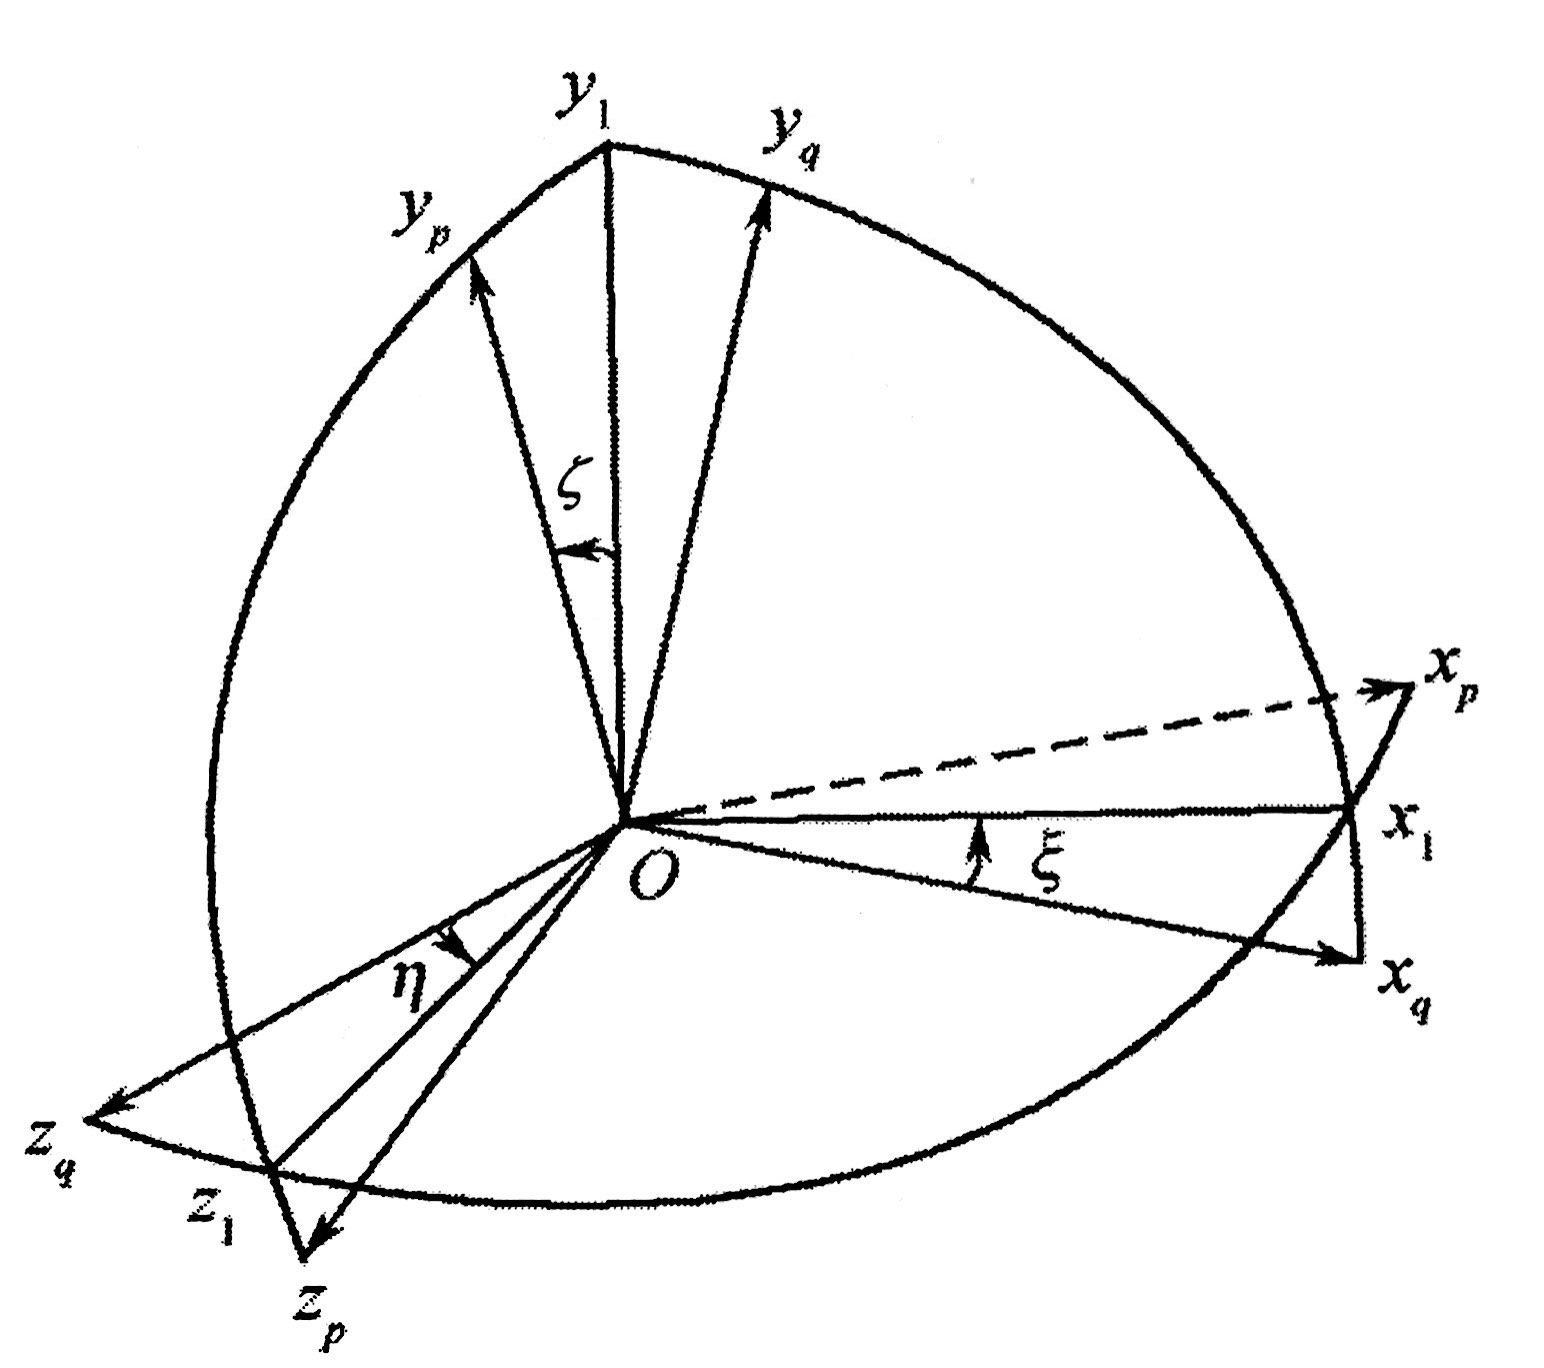
\includegraphics[width=0.3\linewidth]{pic/欧拉角.jpg}
	\caption{坐标系旋转转换}
	\label{欧拉角}
\end{figure}

例如,如图\ref{欧拉角}所示,$o-\bm{x}_q\bm{y}_q\bm{z}_q$分别绕$z,y,x$轴旋转三次,得到
\begin{equation*}
	\begin{split}
		o-\bm{x}_q\bm{y}_q\bm{z}_q \, \xrightarrow{\quad \textstyle M_z[\xi] \quad } o - x_1 y_1 \bm{z}_q \, \xrightarrow{\quad \textstyle M_y[\eta] \quad } o - \bm{x}_p y_1 \bm{z}_1\ \, \xrightarrow{\quad \textstyle M_x[\zeta] \quad } \,o - \bm{x}_p \bm{y}_p \bm{z}_p
	\end{split}
\end{equation*}
即
\begin{equation}
	P_Q = M_x[\xi] \cdot  M_y[\eta]\cdot  M_z[\zeta]
\end{equation}
进一步代入,得
\begin{equation}
	P_Q = 
	\begin{bmatrix}
		\cos \xi \cos \eta & \sin \xi \cos \eta & - \sin \eta \\
		\cos \xi \sin \eta \sin \zeta - \sin \xi \cos \zeta & \sin \xi \sin \eta \sin \zeta + \cos \xi \cos \zeta & \cos \eta \sin \zeta \\
		\cos \xi \sin \eta \cos \zeta + \sin \xi \sin \zeta & \sin \zeta \sin \eta \cos \zeta - \cos \xi \sin \zeta & \cos \eta \cos \zeta
	\end{bmatrix}
\end{equation}

\subsection{坐标间矢量导数的关系}
\vspace*{-1em}
\defination[矢量导数]
{
	\dy[矢量导数]{SLDS}:同一矢量在不同坐标系有不同的投影,其导数的数值不同。
}

设坐标系$O:o-xyz$相对于坐标系$P:o_p-x_py_pz_p$有角速率$\omega.$ 矢量$\bm{a}$在坐标系$O$的投影为
\begin{equation}
	\bm{a} = a_x \bm{x}^0 + a_y \bm{y}^0 + a_z \bm{z}^0
\end{equation}
取微分,得
\begin{equation}
	\dfrac{\d \bm{a}}{\d t} = \dfrac{\d a_x}{\d t}\bm{x}^0 + \dfrac{\d a_y}{\d t} \bm{y}^0 + \dfrac{\d a_z}{\d t} \bm{z}^0 + a_x \dfrac{\bm{x}^0}{\d t} + \dfrac{}{分母}
\end{equation}

\section{常用坐标系及其相互转换}
\subsection{常用坐标系}
常用的坐标系分类
\begin{itemize}
	\item 取地心为原点:地心惯性坐标系,地心固连坐标系\vspace*{-0.5em}
	\item 取发射点为原点:发射坐标系,发射惯性坐标系\vspace*{-0.5em}
	\item 取对象质心为原点:体坐标系,速度坐标系,半速度坐标系
\end{itemize}

\begin{enumerate}
	\item \dy[地心惯性坐标系$I$]{DXGXZBX}:$O_E - X_I Y_I Z_I$(静系)
	\vspace*{1em}
	
	\begin{minipage}{0.6\linewidth}
		\centering
		\setlength{\tabcolsep}{12mm}{
		\begin{tabular}{cl}
			\hline
			原点 & 地心$O_E$\\
			\hline
			$X$轴 & $X_I$:平春分点\\
			\hline
			$Y$轴 & $Y_I$:右手法则\\
			\hline
			$Z$轴 & $Z_I$:地球自转轴\\
			\hline
		\end{tabular}
	}
	\end{minipage}

	\vspace*{1.5em}
	\item \dy[地心坐标系$E$]{DXZBX}:$O_E - X_E Y_E Z_E$(动系)
	\vspace*{1em}
	
	\begin{minipage}{0.6\linewidth}
		\centering
		\setlength{\tabcolsep}{12mm}{
		\begin{tabular}{cl}
			\hline
			原点 & 地心$O_E$\\
			\hline
			$X$轴 & $X_E$:给定子午线\\
			\hline
			$Y$轴 & $Y_E$:右手法则\\
			\hline
			$Z$轴 & $Z_E$:地球自转轴\\
			\hline
		\end{tabular}
	}
	\end{minipage}
	
	\vspace*{1.5em}
	\item \dy[发射坐标系$G$]{FSZBX}:$O - xyz$(动系)
	\vspace*{1em}
	
	\begin{minipage}{0.6\linewidth}
		\centering
		\setlength{\tabcolsep}{8mm}{
			\begin{tabular}{cl}
				\hline
				原点 & 发射点$O$\\
				\hline
				$X$轴 & $x$:发射水平面内指向瞄准方向\\
				\hline
				$Y$轴 & $y$:发射水平面指向上方\\
				\hline
				$Z$轴 & $z$:右手法则\\
				\hline
			\end{tabular}
		}
	\end{minipage}
	\vspace*{0.5em}
	
	对于球模型:$\varphi_0$:地心纬度,$\alpha_0$:发射方位角。\\
	对于椭球模型:$\varphi_0$:地心纬度,$\alpha_0$:发射方位角。
	
	\item \dy[发射惯性坐标系$A$]{FSGXZBX}:$O_A - x_A y_A z_A$(静系)
	\vspace*{1em}
	
	\begin{minipage}{0.6\linewidth}
		\centering
		\setlength{\tabcolsep}{8mm}{
			\begin{tabular}{cl}
				\hline
				原点 & 发射点$O_A$,起飞瞬间与发射点$O$重合\\
				\hline
				$X$轴 & $x_A$:起飞瞬间的发射水平面内指向瞄准方向\\
				\hline
				$Y$轴 & $y_A$:起飞瞬间的发射水平面指向上方\\
				\hline
				$Z$轴 & $z_A$:右手法则\\
				\hline
			\end{tabular}
		}
	\end{minipage}
	
	\vspace*{1.5em}
	\item \dy[平移坐标系$A$]{PYZBX}:$o_T - x_T y_T z_T$(动系)
	\vspace*{1em}
	
	\begin{minipage}{0.6\linewidth}
		\centering
		\setlength{\tabcolsep}{8mm}{
			\begin{tabular}{cl}
				\hline
				原点 & 发射点$O_A$,起飞瞬间与发射点$O$重合\\
				\hline
				$X$轴 & $x_A$:起飞瞬间的发射水平面内指向瞄准方向\\
				\hline
				$Y$轴 & $y_A$:起飞瞬间的发射水平面指向上方\\
				\hline
				$Z$轴 & $z_A$:右手法则\\
				\hline
			\end{tabular}
		}
	\end{minipage}
	
	\vspace*{1.5em}
	\item \dy[弹体坐标系$B$]{DTZBX}:$o_1 - x_1 y_1 z_1$(动系)
	\vspace*{1em}
	
	\begin{minipage}{0.6\linewidth}
		\centering
		\setlength{\tabcolsep}{8mm}{
			\begin{tabular}{cl}
				\hline
				原点 & 弹体质心$O_1$\\
				\hline
				$X$轴 & $x_1$:沿弹体对称轴指向头部\\
				\hline
				$Y$轴 & $y_1$:位于主对称面内,垂直于$X$轴\\
				\hline
				$Z$轴 & $z_1$:右手法则,顺着发射方向看向右为正\\
				\hline
			\end{tabular}
		}
	\end{minipage}
	
	\vspace*{1.5em}
	\item \dy[速度坐标系$V$]{SDZBX}:$o_1 - x_v y_v z_v$(动系)
	\vspace*{1em}
	
	\begin{minipage}{0.6\linewidth}
		\centering
		\setlength{\tabcolsep}{8mm}{
			\begin{tabular}{cl}
				\hline
				原点 & 弹体质心$O_1$\\
				\hline
				$X$轴 & $x_v$:弹体的速度方向\\
				\hline
				$Y$轴 & $y_v$:位于主对称面内,垂直于$X$轴\\
				\hline
				$Z$轴 & $z_v$:右手法则\\
				\hline
			\end{tabular}
		}
	\end{minipage}

	\vspace*{1.5em}
	\item \dy[半速度坐标系$H$]{BSDZBX}:$o_1 - x_h y_h z_h$(动系)
	\vspace*{1em}
	
	\begin{minipage}{0.6\linewidth}
		\centering
		\setlength{\tabcolsep}{5mm}{
			\begin{tabular}{cl}
				\hline
				原点 & 弹体质心$O_1$\\
				\hline
				$X$轴 & $x_h$:弹体的速度方向\\
				\hline
				$Y$轴 & $y_h$:包含速度矢量的铅锤面内垂直于$x_h$,向上为正\\
				\hline
				$Z$轴 & $z_h$:右手法则\\
				\hline
			\end{tabular}
		}
	\end{minipage}
\end{enumerate}

\subsection{各坐标系间的转换关系}
\begin{enumerate}
	\item $I \to E$:$Z$轴重合,$X$轴处于赤道面内相差角$\varOmega_G = \omega_e \cdot t$(时角),则转换矩阵为
	\begin{equation}
		E_I = M_z [\varOmega_G]
	\end{equation}
	
	\item $E \to G$:设地球为圆球,发射点可用经纬度$(\lambda_0, \varphi_0)$来描述,即
	\begin{equation}
		G_E = M_y\big[-(90\degree + \alpha_0)\big]\cdot M_x[\varphi_0] \cdot M_z \big[-(90 \degree - \lambda_0)\big]
	\end{equation}

	\item $G \to B$:设$G \to B$转序为$321$,旋转角为$\varphi, \psi ,\gamma$,则
	\begin{equation}
		B_G = M_x[\gamma]\cdot M_y[\psi] \cdot M_z[\varphi]
	\end{equation}
	\hspace*{1em}\defination[新的欧拉角{\RMN[1]}]
	{
		\dy[俯仰角$\varphi$]{FYJ}:轴$ox_1$在发射面$xoy$上的投影与$x$的夹角,投影在$x$的上方为正。\\
		\hspace*{2.2em}\dy[偏航角$\psi$]{PHJ}:轴$ox_1$与发射面$xoy$的夹角,$ox_1$在发射面左边为正。\\
		\hspace*{2.2em}\dy[滚动角$\gamma$]{GDJ}:旋转角速度矢量与$ox_1$轴方向一致时为正。
	}

	\item $G \to V$:设$G \to V$转序为$321$,旋转角为$\theta, \sigma ,\nu$,则
	\begin{equation}
		V_G = M_x[\nu]\cdot M_y[\sigma] \cdot M_z[\theta]
	\end{equation}
	\hspace*{1em}\defination[新的欧拉角{\RMN[2]}]
	{
		\dy[速度倾角$\theta$]{SDQJ}:轴$ox_v$在发射面$xoy$上的投影与$x$的夹角,投影在$x$的上方为正。\\
		\hspace*{2.2em}\dy[航迹偏航角$\sigma$]{HJPHJ}:轴$ox_v$与发射面$xoy$的夹角,$ox_v$在发射面左边为正。\\
		\hspace*{2.2em}\dy[倾侧角$\nu$]{QCJ}:旋转角速度矢量与$ox_v$轴方向一致时为正。
	}

	
	\item $V \to B$:由于速度系$y_v$轴位于主对称面内,因此$V \to B$只有两个欧拉角,设为$\alpha,\beta$,设定$V \to B$的转序为23,则
	\begin{equation}
		B_V = M_z[\alpha] \cdot M_y [\beta]
	\end{equation}
	
	\hspace*{1em}\defination[新的欧拉角{\RMN[3]}]
	{
		\dy[测滑角$\beta$]{CHJ}:速度轴$x_v$与弹体主对称面的夹角,右方为正。\\
		\hspace*{2.2em}\dy[攻角$\alpha$]{GJ}:速度轴$x_v$与在主对称面投影与弹体纵轴的夹角,下方为正。
	}
	
	
	\item $A \to G$:由于在发射时刻$A,G$坐标系重合,因此其转换角与飞行时间$t$相关,发射系绕地轴旋转角为$\omega_e t$,则
	\begin{equation}
		G_A = M_y[-\alpha_0] \cdot M_z[-\phi_0] \cdot M_x[\omega_e t] \cdot M_z[\phi_0] \cdot M_y[\alpha_0]
	\end{equation}
	如果火箭飞行时间较短,认为$\omega_e t$为小量,在转换矩阵中取其一次项,则
	\begin{equation}
		G_A = 
		\begin{bmatrix}
			1 & \omega_{ez}t & -\omega_{ey} t\\
			-\omega_{ez}t & 1 &\omega_{ex} t \\
			\omega_{ey} t & -\omega_{ex}t & 1 
		\end{bmatrix}
	\end{equation}
	其中,
	\begin{equation}
		\begin{cases}
			\,\omega_{ex} = \omega_e \cos \phi_0 \cos \alpha_0 \\
			\,\omega_{ey} = \omega_e \sin \phi_0\\
			\,\omega_{ez} = - \omega_e \cos \phi_0 \sin \alpha_0
		\end{cases}
	\end{equation}
\end{enumerate}

\subsection{常用欧拉角的联系方程}
由于各坐标系之间定义有欧拉角,必然存在一定的联系。

\begin{enumerate}
	\item \textbf{$B,G,V$之间的联系}
	\begin{equation}
		V_G[\theta, \sigma, \nu] = V_B [\alpha, \beta] \cdot B_G [\varphi, \psi, \gamma]
	\end{equation}
	利用姿态角$\varphi, \psi ,\gamma$和攻角侧滑角$\alpha, beta$来确定速度角$\theta, \sigma , \nu$.如果侧向角为小量,则
	\begin{equation}
		\begin{cases}
			\, \sigma= \psi \cos \alpha + \gamma \sin \alpha - \beta \\
			\, \nu = - \psi \sin \alpha + \gamma \cos \alpha \\
			\, \theta = \varphi - \alpha
		\end{cases}
	\end{equation}
	若功角$\alpha$也为小量,则
	\begin{equation}
		\begin{cases}
			\, \theta= \varphi - \alpha \\
			\, \sigma = \psi - \beta \\
			\, \nu = \gamma
		\end{cases}
	\end{equation}

\item \textbf{$B,G,V$之间的联系}\\
	\hspace*{2em}弹体相对发射系姿态角为$\varphi, \psi, \gamma$,相对平移系姿态角为$\varphi_T, \psi_T, \gamma_T$,相对系与发射惯性系矩阵$G_T$,有
	\begin{equation}
		B_T[\varphi_T, \psi_T, \gamma_T] = B_G [\varphi, \psi, \gamma] \cdot G_T[\alpha_0, \phi_0, \omega_e t]
	\end{equation}
	由此可利用姿态角$\varphi,\psi, \gamma $和飞行时间$t$来确定惯性姿态角$\varphi_T, \psi_T, \gamma_T$。如果认为侧向角及时间为小量,则
	\begin{equation}
		\begin{cases}
			\, \varphi_T = \varphi + \omega_{ez}t\\
			\, \psi_T = \psi + (\omega_{ey}\cos \varphi - \omega_{ex}\sin \varphi)\cdot t\\
			\, \gamma_t = \gamma + (\omega_{ey} \sin \varphi + \omega_{ex}\cos \varphi)\cdot t
		\end{cases}
	\end{equation}

\end{enumerate}

\section{变质量力学基本原理}
\subsection{变质量质点基本方程}
	\textbf{1. 火箭质量}
	
	由于发动机工作,飞行中有大量质点从发动机中喷出,因此必须规定一个表面,以此表面内质量作为火箭的总质量。通常此表面取为火箭外表面和发动机喷口断面。因此火箭是一个存在质点流动的变质量物体。
	
	\vspace*{1em}
	\textbf{2. 变质量质点基本方程}
	
	设当前质量为$m(t)$,当前绝对速度为$\bm{V}$,则其动量为
	\begin{equation}
		\bm{Q}(t) = m(t) \cdot \bm{V}
	\end{equation}
	质点在$\d t$时间内,有外界作用力$\bm{F}$,且向外以相对速度$\bm{V}_r$喷射质量元$-\d m$。设质点速度变化为$\d \bm{V}$,则有
	\begin{equation}
		\begin{split}
			\bm{Q}(t+\d t) &= \big(m - (-\d m)\big)\cdot \big(\bm{V} + \d \bm{V}\big)+(-\d m) \cdot (\bm{V} + \bm{V}_r)\\
			& = m(t)(\bm{V} + \d \bm{V}) - \d m \bm{V}_r
		\end{split}
	\end{equation}
	则
	\begin{equation}
		\begin{split}
			\d \bm{Q} &= \bm{Q}(t + \d t) - \bm{Q}(t) \\
			&= m(\bm{V} + \d \bm{V}) - \d m \bm{V}_r - m \cdot \bm{V} \\
			& = m \d \bm{V} -\d m \bm{V}_r
		\end{split}
	\end{equation}
	对常质量质点有动量定律
	\begin{equation}
		\d \bm{Q} = \bm{F} \d t
	\end{equation}
	所以
	\begin{equation}
		\bm{F} \d t = m \d \bm{V} -\d m \bm{V}_r
	\end{equation}
	由此可以得到
	
	\theorem[变质量质点基本方程(密歇尔斯基方程)\index{BZLZDJBFC@变质量质点基本方程}\index{MXESJFC@密歇尔斯基方程}]
	{
		\vspace*{-1em}
		\begin{equation}
			m \dfrac{\d \bm{V}}{\d t} = \bm{F}+\dfrac{\d m}{\d t} \bm{V}_r = \bm{F} + \textcolor{red}{\bm{P}_r}
		\end{equation}
		其中,$\bm{F}$为牛顿第二定律的外力;$\textcolor{red}{\bm{P}_r}$为喷射反作用力,加速力。
	}
	假设质点不受外力作用,且假设有$\bm{V}_r$与$\bm{V}$反向,则
	\begin{equation}
		m \dfrac{\d v}{\d t} = - \dfrac{\d m}{\d t} v_r \quad \Rightarrow \quad \d v = - \d v_r \dfrac{\d m}{m}
	\end{equation}
	再假设质量元喷射速度为常值,则有质点速度为
	\begin{equation}
		v = v_0 + v_r \ln \dfrac{m_0}{m}
	\end{equation}
	设初始速度为0,则可以得到
	
	\theorem[齐奥尔科夫斯基公式\index{QAEKFSJGS@齐奥尔科夫斯基公式}]
	{
		\quad \vspace*{-1em}
		\begin{equation}
			v_k = v_r \ln \dfrac{m_0}{m_k}
		\end{equation}
		设\dy[结构比]{JGB}为$\mu_k = \dfrac{m_k}{m_0}$,则
		\begin{equation}
			v_k = -v_r \ln \mu_k
		\end{equation}
		其中,$v_k$为理想速度。
	}

\subsection{变质量质点系的运动方程}
	对于变质量质点系,除了质点随物体作牵连运动外,在物体内部还有相对运动,会对物体运动有影响,应用密歇尔斯基方程存在近似性。
	
	在惯性参考系内,质点系总外力为$\bm{F}_s$,总力矩为$\bm{M}_s$,则运动方程为
	\begin{align}
		\bm{F}_s &= \sum_{i=1}^N m_i \dfrac{\d^2 \bm{r}_i}{\d t^2} \\[0.5em]
		\bm{M}_s &= \sum_{i=1}^N m_i\bm{r}_i \times \dfrac{\d^2 \bm{r}_i}{\d t^2} 
	\end{align}
	对于连续质点系(物体)的运动方程,则有
	\begin{align}
		\bm{F}_s &= \int_m \dfrac{\d^2 \bm{r}}{\d t^2} \, \d m \label{相对牛二}\\[0.5em]
		\bm{M}_s &= \int_m \bm{r} \times \dfrac{\d^2 \bm{r}}{\d t^2} \, \d m
	\end{align}

	\textbf{1. 质心运动方程}
	
	任一质点在惯性系中的矢径为
	\begin{equation}
		\bm{r} = \bm{r}_{c.m} + \bm{\rho}
	\end{equation}
	其中$\bm{r}_{c.m}$为质心的矢径,$\bm{\rho}$是相对位置矢径,则有绝对加速度为
	\begin{equation}
		\dfrac{\d^2 \bm{r}}{\d t^2} = \dfrac{\d^2 \bm{r}_{c.m}}{\d t^2} + 2 \bm{\omega}_T \times \dfrac{\delta \bm{\rho}}{\delta t} + \dfrac{\delta^2 \bm{\rho}}{\delta t^2} + \dfrac{\bm{\omega}_T}{\d t}\times \bm{\rho} + \bm{\omega}_T \times (\bm{\omega}_T \times \bm{\rho}) 
		\label{绝对加速度}
	\end{equation}
	将\eqref{绝对加速度}代入\eqref{相对牛二},可以得到
	\begin{align*}
		\bm{F}_s & = \int_m \Bigg[\dfrac{\d \bm{r}_{c.m}}{\d t^2} + 2 \bm{\omega}_T \times \dfrac{\delta \bm{\rho}}{\delta t} + \dfrac{\delta^2 \bm{\rho}}{\delta t^2} + \dfrac{\bm{\omega}_T}{\d t}\times \bm{\rho} + \bm{\omega}_T \times (\bm{\omega}_T \times \bm{\rho}) \Bigg]\,\d m \\[0.5em]
		& = m \dfrac{\d^2 \bm{r}_{c.m}}{\d t^2} + 2 \bm{\omega}_T \times \int_m \dfrac{\delta \bm{\rho}}{\delta t}\, \d m + \int_m \dfrac{\delta^2 \bm{\rho}}{\delta t^2}\, \d m + \bm{\omega}_T \times \left(\bm{\omega}_T \times \int_m \bm{\rho}\, \d m \right)
	\end{align*}
由质心的定义,有$\displaystyle \int_m \bm{\rho} \, \d m = 0$,则可以得到

\theorem[任意变质量物体的一般运动方程]
{
	 \vspace*{-1em}
\begin{equation}
	\bm{F}_S = m \dfrac{\d^2 \bm{r}_{c.m}}{\d t^2} + 2 \bm{\omega}_T \times \int_m \dfrac{\delta \bm{\rho}}{\delta t}\, \d m + \int_m \dfrac{\delta^2 \bm{\rho}}{\delta t^2}\, \d m 
\end{equation}
}

\noindent 相应地可以得到

\theorem[任意变质量物体的质心运动方程]
{
	\vspace*{-1em}
	\begin{equation}
		m \dfrac{\d^2 \bm{r}_{c.m}}{\d t^2}  = \bm{F}_s + \bm{F}'_{k} + \bm{F}'_{rel} 
		\label{运动方程}
	\end{equation}
	其中,
	{
		\begin{enumerate}[\hspace*{2em}]
			\item \dy[附加哥氏力]{FJGSL}\quad $\displaystyle \bm{F}'_k = - 2 \bm{\omega}_T \times \int_m \dfrac{\delta \bm{\rho}}{\delta t}\, \d m$
			\item \dy[附加相对力]{FJXDL} \quad $\displaystyle \bm{F}'_{rel} = - \int_m \dfrac{\delta^2 \bm{\rho}}{\delta t^2}\, \d m$
		\end{enumerate}
	}
}

\textbf{2. 绕质心运动方程}

系统$S$绕质心的力矩方程为
\begin{equation}
	\bm{M}_{c.m} = \int_m \bm{\rho} \times \dfrac{\d^2 \bm{r}}{\d t^2} \, \d m
\end{equation}
将加速度的表达式\eqref{绝对加速度}代入,可以得到
\begin{align*}
	\bm{M}_{c.m} = \int_m \bm{\rho} \times \dfrac{\d^2 \bm{r}_{c.m}}{\d t^2}\, \d m 
	+ 2 \int_m \bm{\rho} \times \left(\bm{\omega}_T \times \dfrac{\delta \bm{\rho}}{\delta t}\right)\, \d m 
	+ \int_m \bm{\rho} \times \dfrac{\delta^2 \bm{\rho}}{\delta t^2}\, \d m 
	+ \int_m \bm{\rho}\times \left(\dfrac{\d \bm{\omega}_T}{\d t} \times \bm{\rho}\right)\, \d m 
	+ \int_m \bm{\rho}\times \big[\bm{\rho} \times (\bm{\omega}_T \times \bm{\rho})\big]\, \d m
\end{align*}

由于质心的定义,$\displaystyle \int_m \bm{\rho} \, \d m = 0$且$\dfrac{\d^2 \bm{r}_{c.m}}{\d t^2}$与质量无关,所以$\displaystyle \int_m \bm{\rho} \times \dfrac{\d^2 \bm{r}_{c.m}}{\d t^2}\, \d m = 0$,即化简为
\begin{align}
	\bm{M}_{c.m} = 2 \int_m \bm{\rho} \times \left(\bm{\omega}_T \times \dfrac{\delta \bm{\rho}}{\delta t}\right)\, \d m 
	+ \int_m \bm{\rho} \times \dfrac{\delta^2 \bm{\rho}}{\delta t^2}\, \d m 
	+ \int_m \bm{\rho}\times \left(\dfrac{\d \bm{\omega}_T}{\d t} \times \bm{\rho}\right)\, \d m 
	+ \int_m \bm{\rho}\times \big[\bm{\rho} \times (\bm{\omega}_T \times \bm{\rho})\big]\, \d m
	\label{转动方程}
\end{align}
记
\begin{align*}
	\bm{M}'_k &= - 2 \int_m \bm{\rho} \times \left(\bm{\omega}_T \times \dfrac{\delta \bm{\rho}}{\delta t}\right)\, \d m \\[0.5em]
	\bm{M}'_{rel} &= - \int_m \bm{\rho} \times \dfrac{\delta^2 \bm{\rho}}{\delta t^2}\, \d m
\end{align*}
则\eqref{转动方程}可以写为
\begin{equation}
	\int_m \bm{\rho}\times \left(\dfrac{\d \bm{\omega}_T}{\d t} \times \bm{\rho}\right)\, \d m 
	+ \int_m \bm{\rho}\times \big[\bm{\rho} \times (\bm{\omega}_T \times \bm{\rho})\big]\, \d m 
	= \bm{M}_{c.m} + \bm{M}'_k + \bm{M}'_{rel}
	\label{转动方程2}
\end{equation}
公式\eqref{转动方程2}左端第二项可以处理为
\begin{equation}
	\int_m \bm{\rho} \times \big[\bm{\omega}_T \times (\bm{\omega}_T \times \bm{\rho})\big]\, \d m = \bm{\omega}_T \times \int_m \bm{\rho} \times (\bm{\omega}_T \times \bm{\rho}) \, \d m \xlongequal[]{ \textstyle \hspace*{0.5em} \Delta \hspace*{0.5em}} \bm{\omega}_T \times \bm{H}_{c.m}
\end{equation}
其中$\bm{H}_{c.m}$为将系统视为刚体后,刚体对质心的角动量。

建立与物体固连的坐标系$o_1 - xyz$,有
\begin{equation*}
	\bm{\omega}_T = 
	\begin{bmatrix}
		\omega_{Tx} & \omega_{Ty} & \omega_{Tz}
	\end{bmatrix}^{\text{T}} \qquad \bm{\rho} = 
\begin{bmatrix}
	x & y & z
\end{bmatrix}^{\text{T}}
\end{equation*}
则角动量为
\begin{align*}
	\bm{H}_{c.m} & = \int_m \big[\bm{\rho} \times (\bm{\omega}_T \times \bm{\rho})\big]\, \d m 
	= \int_m \big[(\bm{\rho \cdot \bm{\rho}}) \bm{\omega}_T - (\bm{\rho \cdot \bm{\omega_T}})\bm{\rho }\big]\, \d m\\[0.5em]
	& = \int_m \big[(\bm{\rho}\cdot \bm{\rho})\bm{\omega}_T - (\bm{\rho} \cdot \bm{\rho}^{\text{T}})\bm{\omega}_T\big]\, \d m\\[0.5em]
	& = \int_m 
	\begin{bmatrix}
		y^2 + z^2 & -xy & -xz \\
		-xy & z^2 + x^2 & -yz \\
		-zx & -zy & x^2 + y^2 
	\end{bmatrix}
	\,
	\begin{bmatrix}
		\omega_{Tx}\\
		\omega_{Ty}\\
		\omega_{Tz}
	\end{bmatrix}
	\, \d m\\
	& =  \bm{I}\cdot \bm{\omega}_T
\end{align*}

其中,$\bm{I}$为\dy[惯性张量]{GXZL}
\begin{equation}
	\bm{I} = 
	\begin{bmatrix}
		I_{xx} & - I_{xy} & -I_{xz} \\
		-I_{xy} & I_{yy} & -I_{yz} \\
		-I_{zx} & -I_{zy} & I_{zz}
	\end{bmatrix}
\end{equation}

定义\dy[转动惯量]{ZDGL}$I_{xx},I_{yy},I_{zz}$和\dy[惯量积]{GLJ}
\begin{equation}
	\begin{cases}
		\, \displaystyle I_{xx} = \int_m(y^2 + z^2)\, \d m \\[0.8em]
		\, \displaystyle I_{yy} = \int_m(x^2 + z^2)\, \d m \\[0.8em]
		\,  \displaystyle I_{zz} = \int_m(y^2 + x^2)\, \d m \\[0.8em]
		\,  \displaystyle I_{xy} = I_{yx} = \int_m xy \, \d m\\[0.8em]
		\,  \displaystyle I_{xz} = I_{zx} = \int_m xz \, \d m\\[0.8em]
		\,  \displaystyle I_{xy} = I_{yx} = \int_m yz \, \d m
	\end{cases}
\end{equation}
则
\begin{equation}
	\bm{H}_{c.m} = \int_m \bm{\rho} \times (\bm{\omega}_T \times \bm{\rho})\, \d m =  \bm{I}\cdot \bm{\omega}_T 
	\label{角动量}
\end{equation}

同理可以对方程\eqref{转动方程2}左边第一项处理得到
\begin{equation}
	\int_m \bm{\rho} \times \left(\dfrac{\d \bm{\omega}_T}{\d t} \times \bm{\rho}\right) = \int_m \begin{bmatrix}
		y^2 + z^2 & -xy & -xz \\
		-xy & z^2 + x^2 & -yz \\
		-zx & -zy & x^2 + y^2 
	\end{bmatrix}
	\,
	\begin{bmatrix}
		\dfrac{\d \omega_{Tx}}{\d t}\\[0.8em]
		\dfrac{\d \omega_{Ty}}{\d t}\\[0.8em]
		\dfrac{\d \omega_{Tz}}{\d t}
	\end{bmatrix}
	\, \d m = \bm{I}\cdot \dfrac{\d \bm{\omega}_T}{\d t}
	\label{角动量导}
\end{equation}

则最终的转动方程为

\theorem[任意变质量物体的绕质心运动方程]
{
	\vspace*{-1em}
	\begin{equation}
		\bm{I}\cdot \dfrac{\d \bm{\omega}_T}{\d t} + \bm{\omega}_T\times(\bm{I}\cdot \bm{\omega}_T) = \bm{M}_{c.m}+\bm{M}'_k+\bm{M}'_{rel}
		\label{绕质心的运动方程}
	\end{equation}
	其中,
	{
		\begin{enumerate}[\hspace*{2em}]
			\item \dy[附加哥氏力矩]{FJGSLJ}\quad $\displaystyle \bm{M}'_k = -2 \int_m \bm{\rho}\times \left(\bm{\omega}_T \times \dfrac{\delta \bm{\rho}}{\delta t}\right)\, \d m$
			\item \dy[附加相对力矩]{FJXDLJ} \quad $\displaystyle \bm{F}'_{rel} = - \int_m \bm{\rho} \times \dfrac{\delta^2 \bm{\rho}}{\delta t^2} \, \d m$
			\item \dy[惯量张量]{GXZL} \quad $\displaystyle \bm{I} = 
			\int_m \begin{bmatrix}
				y^2 + z^2 & -xy & -xz \\
				-xy & z^2 + x^2 & -yz \\
				-zx & -zy & x^2 + y^2 
			\end{bmatrix} =
		\begin{bmatrix}
			I_{xx} & - I_{xy} & -I_{xz} \\
			-I_{xy} & I_{yy} & -I_{yz} \\
			-I_{zx} & -I_{zy} & I_{zz}
		\end{bmatrix}$
		\end{enumerate}
	}
}
\vspace*{1em}

\textbf{3. 钢化原理}

\theorem[钢化原理]
{
	一般情况下,任意变质量系统的运动方程,可用一个刚体的运动方程表示。这个刚体的质量等于系统瞬时质量,其受力除真实的外力与外力矩外,还要加上两个附加力和两个附加力矩。
}





























